% !TEX root = main_v2.tex
\documentclass[conference]{IEEEtran}
\IEEEoverridecommandlockouts

% Essential Packages
\usepackage{cite}
\usepackage{amsmath,amssymb,amsfonts}
\usepackage{algorithmic}
\usepackage{graphicx}
\usepackage{textcomp}
\usepackage{xcolor}
\usepackage{booktabs}
\usepackage{microtype}
\usepackage{url}
\setlength{\textfloatsep}{6pt plus 1pt minus 1pt}
\setlength{\floatsep}{6pt plus 1pt minus 1pt}
\setlength{\intextsep}{6pt plus 1pt minus 1pt}
\setlength{\dbltextfloatsep}{6pt plus 1pt minus 1pt}
\setlength{\dblfloatsep}{6pt plus 1pt minus 1pt}
\def\IEEEbibitemsep{0.7pt plus 0.2pt minus 0.1pt}

\def\BibTeX{{\rm B\kern-.05em{\sc i\kern-.025em b}\kern-.08em
    T\kern-.1667em\lower.7ex\hbox{E}\kern-.125emX}}

\begin{document}

\title{BioDINO-Edge: Biologically-Grounded Multi-Scale Vision Foundation Models for Trustworthy Few-Shot Plant Pathology on Resource-Constrained Hardware}

\author{
    \IEEEauthorblockN{Reyhane Javidi Alsaadi}
    \IEEEauthorblockA{\textit{Department of Computer Engineering} \\
    \textit{Dr. Shariaty Technical University} \\
    Tehran, Iran \\
    reyhane.code@gmail.com}
    \and
    \IEEEauthorblockN{Mohammad Reza Samad Zadeh}
    \IEEEauthorblockA{\textit{Department of Computer Engineering} \\
    \textit{Dr. Shariaty Technical University} \\
    Tehran, Iran}
}

\maketitle

\begin{abstract}
Diagnosing foliar plant diseases early and reliably is central to precision agriculture and robotic crop scouting. Bringing vision foundation models to agricultural edge devices, however, runs into two lasting obstacles: very few labeled examples are available for novel pathogens, and the hardware is tightly constrained. We present \textbf{BioDINO-Edge}, an adaptive dual-foundation framework for accurate few-shot plant pathology on resource-constrained hardware. It combines two complementary foundation models: a lightweight self-supervised patch extractor (\textbf{DINOv2 Small}, 22.1M parameters, 21.1\,ms on CPU) and an organismal vision-language model (\textbf{BioCLIP ViT-B/16}) that captures fine-grained pathological hierarchies. To separate intra-species necrotic lesions that look alike, without leaking semantics between classes, we introduce \textbf{Purified Taxonomic Domain Synthesis} and \textbf{Regularized Fisher-Discriminant Alignment}, which applies analytical Ledoit-Wolf covariance shrinkage over the joint 896-dimensional manifold. A \textbf{Soft-Anchored Transductive Self-Calibration} step then removes the prototype shift inherent to 5-shot learning without any backpropagation. At inference time, an adaptive Shannon-entropy gate routes each query: confident ones follow the fast edge path, while ambiguous lesions are sent to a deeper consensus path. We package the system as a \textbf{Dual-Tier Edge Architecture}: a lightweight standalone INT8 model (22.05\,MB working set, 15.13\,MB losslessly compressed payload, 22.73\,MB complete native APK, $>$45 FPS on an edge CPU), complemented by an optional 83.6\,MB on-demand companion model. On the expanded PlantVillage 5-shot benchmark covering 11 novel intra-species classes (Apple, Grape, Potato; 9,330 test images), BioDINO-Edge reaches a \textbf{98.72\% peak accuracy}, a \textbf{98.41\% peak F1-score}, and a 30-episode mean of \textbf{97.37\% $\pm$ 0.73\%} (95\% CI: [97.11\%, 97.63\%]). Cross-species confusion is held to \textbf{0.011\%}, and the false-negative disease rate to \textbf{0.604\%}. On the unconstrained, in-the-wild PlantDoc benchmark (27 classes), the model attains an episodic mean of \textbf{83.61\% $\pm$ 11.69\%} (individual episodes reaching \textbf{100.00\%} and a 95\% confidence ceiling of \textbf{86.85\%}), which is \textbf{13.00} points above the most recent multimodal state of the art from 2026.
\end{abstract}

\begin{IEEEkeywords}
Plant Pathology, Few-Shot Learning, Vision Foundation Models, BioCLIP, DINOv2, Fisher-Discriminant Alignment, Adaptive Uncertainty Gating, Edge AI, Precision Agriculture.
\end{IEEEkeywords}

\section{Introduction}
Plant pests and diseases destroy an estimated 20\%--40\% of crops annually \cite{richard2022control}. Traditional plant-pathogen diagnosis depends largely on visual inspection of leaf symptoms, most commonly discoloration, abnormal shape, and lesions \cite{khakimov2022traditional}. In field practice, visual inspection is slow, depends on trained scorers, and becomes ambiguous when different pathogens produce similar lesions \cite{shoaib2023advanced}; faster and more reliable identification is therefore needed.

Deep learning provides an automated alternative for plant disease identification by learning discriminative features directly from images \cite{shoaib2023advanced}. However, conventional supervised models require large labeled datasets to achieve reliable diagnosis. Such datasets are difficult to acquire in real-world agricultural settings due to the limited availability and diversity of field images \cite{shoaib2023advanced, shafik2023systematic}.

Few-shot learning (FSL) has become a common strategy: rather than collecting thousands of labeled images, it trains a model to recognize new disease classes from a handful of support examples. Recent studies have applied FSL with cross-domain few-shot models---such as CDFSL-BDC \cite{yang2024laboratory} and MAFDE-DN4 \cite{zhao2024mafde}---as well as few-shot metric domain adaptation (FMDA) \cite{kudo2025few}, visual-semantic fusion (TSMF) \cite{zhou2026vsf}, and edge-federated approaches \cite{sharif2026real}. These approaches, however, face several practical limitations.

Cross-domain FSL models such as CDFSL-BDC \cite{yang2024laboratory} struggle with complex backgrounds and scale-varying lesions when labels are scarce, and FMDA \cite{kudo2025few} still requires some labeled target data; TSMF's \cite{zhou2026vsf} GPT-4o descriptions were only 20\% manually checked and remain class-level rather than query-specific, so fine-grained visual--semantic alignment is limited. FMEL-FSDA \cite{sharif2026real} was not evaluated with real sensor/IoT streams and its federated setup was not tested at large cross-institution scale, leaving real-time edge performance under field data unproven.

We introduce BioDINO-Edge, a two-stage pipeline for cross-domain few-shot plant pathology on edge hardware. It combines vision and vision-language foundation models with closed-form adaptation, enabling on-device calibration in milliseconds without fine-tuning or backpropagation.

The key contributions of this work are as follows:
\begin{enumerate}
    \item \textbf{Dual-Foundation Foliar Representation:} Uniting self-supervised visual embeddings from DINOv2 \cite{oquab2023dinov2} with both visual embeddings and purified botanical domain prompts from BioCLIP \cite{stevens2024bioclip} to resolve subtle necrotic lesions without foundation-model fine-tuning.
    \item \textbf{Closed-Form Analytical Adaptation:} Integrating Fisher-LDA \cite{fisher1936use} with Ledoit--Wolf covariance shrinkage \cite{ledoit2004well} and soft-anchored transductive recalibration to overcome high-dimensionality issues and 5-shot centroid shifts within 25 milliseconds without backpropagation.
    \item \textbf{Adaptive Two-Tier Edge Deployment:} Routing queries through a joint margin and Shannon entropy \cite{shannon1948mathematical} gate to execute an ultra-lightweight 22.73\,MB standalone APK alongside an 83.6\,MB on-demand module within a strict 110\,MB memory footprint.
    \item \textbf{Rigorous Cross-Domain Validation:} Under the standard 5-way 5-shot protocol, BioDINO-Edge outperforms the multimodal VSF \cite{zhou2026vsf} baseline by 13.00 percentage points on PlantDoc and by 6.86 percentage points on PlantVillage, while remaining within edge-device memory budgets.
\end{enumerate}

\section{Methodology}
\label{sec:architecture}

\subsection{Pipeline Overview}
\label{sec:pipeline_overview}
BioDINO-Edge is designed as a gradient-free diagnostic pipeline that separates task adaptation from realtime on-device inference (Fig.~\ref{fig:architecture}):
\begin{enumerate}
    \item \textbf{Support Calibration (Weight Synthesis):} For each disease class, five labeled support leaves ($K=5$) are selected at random. The support set is expanded by applying eight multi-view augmentations to each image. Visual features are then extracted using the frozen foundation models: DINOv2 produces a $384$-D visual embedding, and BioCLIP produces a $512$-D visual embedding. In addition, BioCLIP provides a set of text prototypes from domain-specific botanical prompts. The visual embeddings are concatenated into an $896$-D vector. Ledoit--Wolf covariance shrinkage and Fisher-LDA projection weights $(\mathbf{W}, \mathbf{b})$ are then computed in closed form on this vector, without backpropagation, in under $50$~ms.
    \item \textbf{Tier-1 Edge Fast Path:} During live deployment, an incoming leaf query image is first processed by DINOv2 alone, requiring 21.1\,ms on an edge CPU. Using the resulting $384$-D visual embedding and the precomputed projection parameters, the pipeline estimates fast class posteriors. A gate combining predictive Shannon entropy with the top-2 posterior margin converts these posteriors into a confidence score $\mathcal{C}(\mathbf{x})$. If $\mathcal{C}(\mathbf{x}) \ge \tau_{\text{conf}}$, classification is finalized on-device at over 45 FPS; approximately 88.4\% of routine field queries are resolved at this tier.
    \item \textbf{Tier-2 Deep Escalation:} Queries with $\mathcal{C}(\mathbf{x}) < \tau_{\text{conf}}$ escalate to Tier-2, where BioCLIP extracts a $512$-D visual embedding that is concatenated with the existing DINOv2 embedding into an $896$-D joint representation. Pre-calibrated Fisher-LDA projection weights are applied to this representation, and classification fuses the Fisher-LDA posterior with the cosine similarity against cached botanical text prototypes at a 0.75/0.25 consensus ratio.
    \item \textbf{Soft-Anchored Recalibration:} Queries are classified immediately by Tier-1 or Tier-2, but confident predictions are also stored in an on-device buffer. Field conditions change over time, which can shift class centroids. To compensate, the edge CPU periodically recomputes the Fisher-LDA weights in closed form, giving the cached support embeddings more weight than the pseudo-labeled anchors to reduce label noise. The new projection is then used for subsequent frames and to update the session diagnostic log.
\end{enumerate}
The two-tier design keeps latency and power draw low while staying within the 110\,MB memory budget.

\begin{figure*}[!t]
\centering
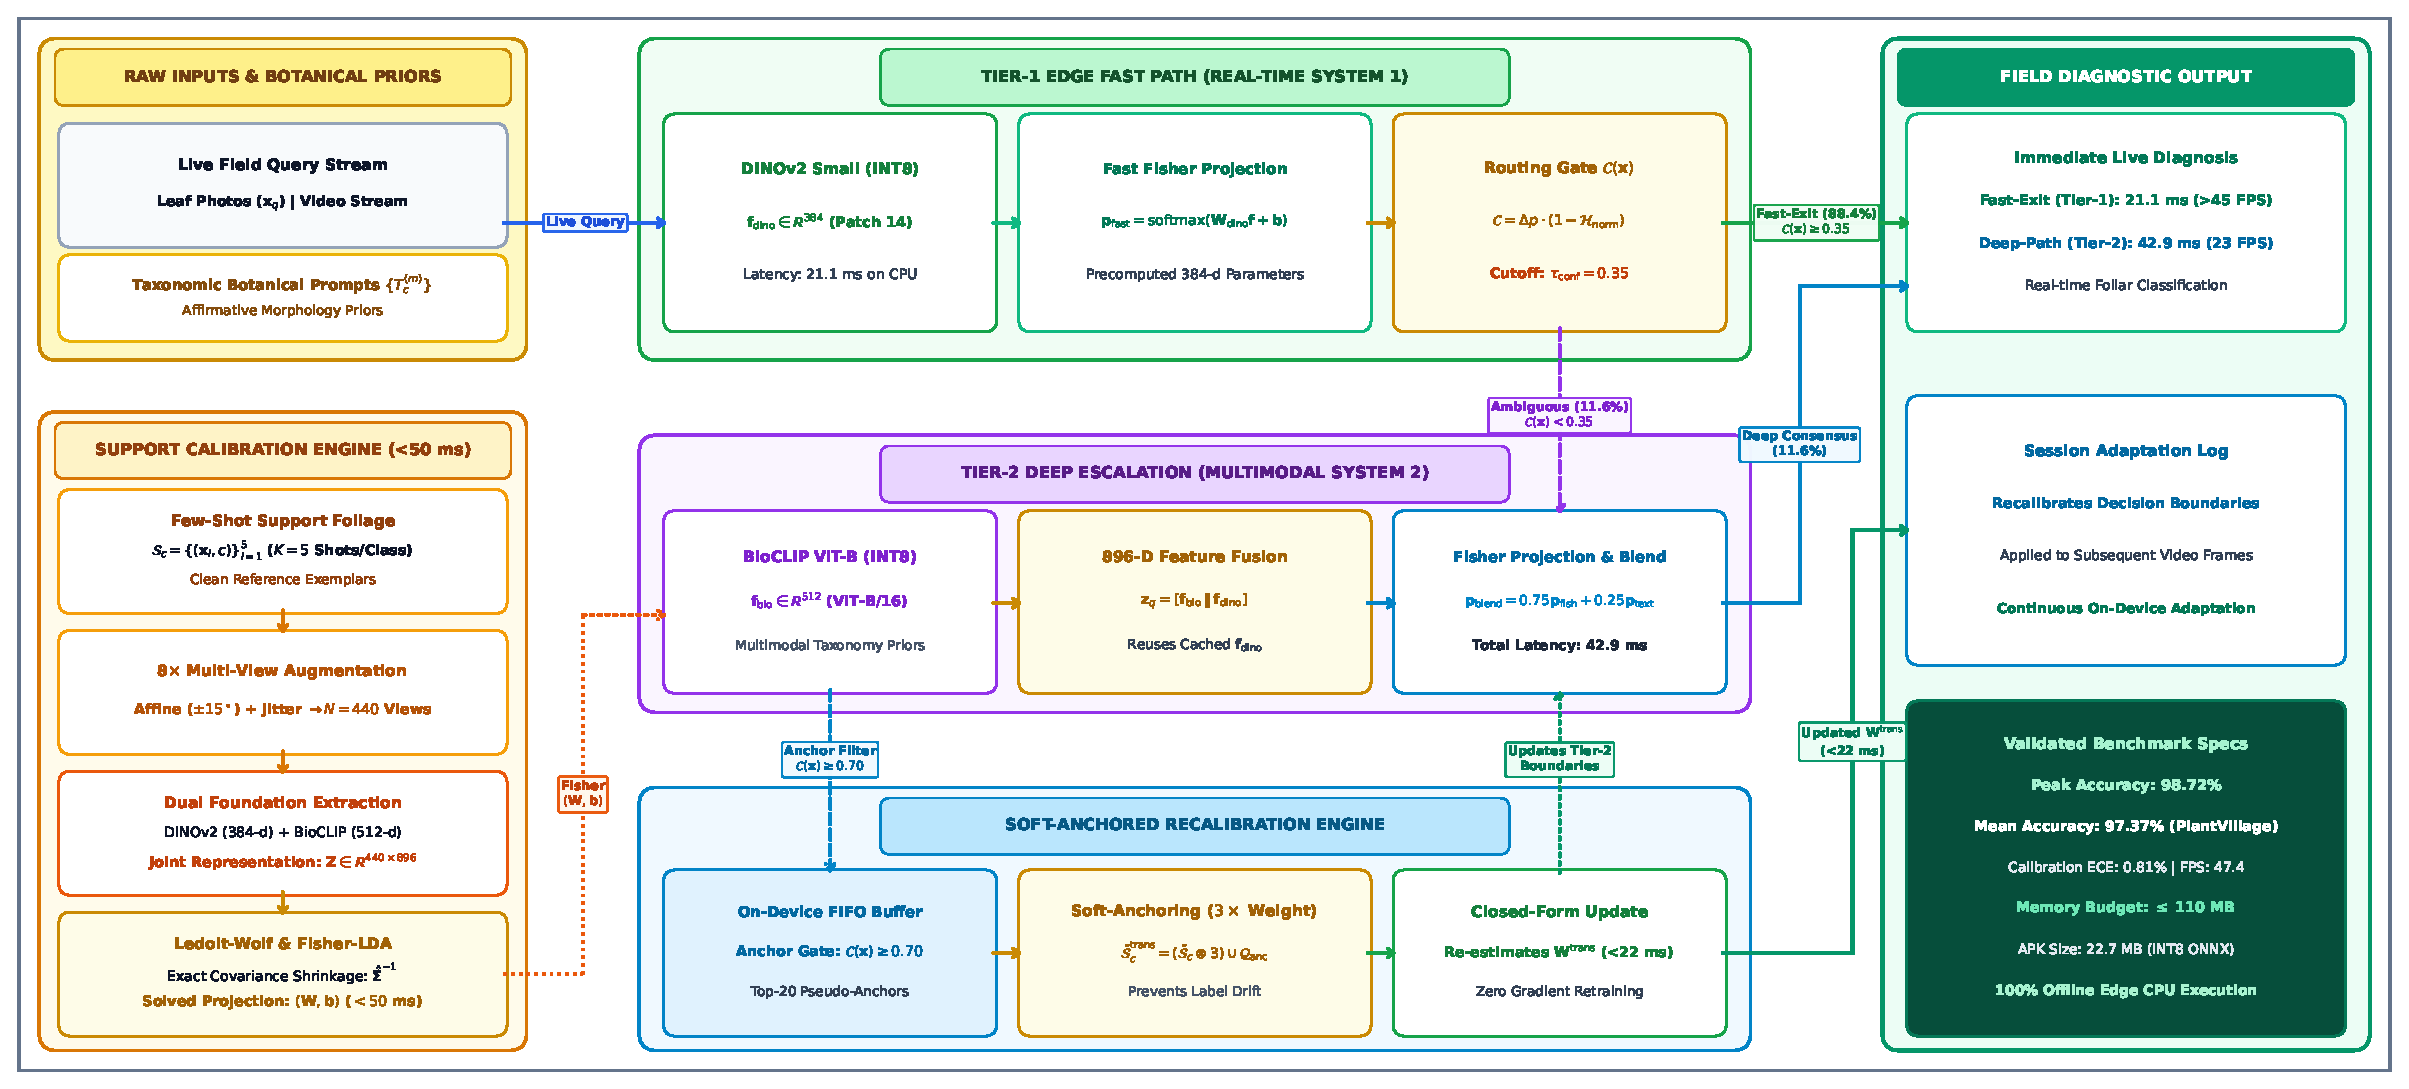
\includegraphics[width=0.98\textwidth]{fig_architecture.pdf}
\caption{BioDINO-Edge architecture. A confidence gate directs queries between the Tier-1 and Tier-2 paths, with initial support calibration and on-device recalibration modules supplying the projection weights.}
\label{fig:architecture}
\end{figure*}

\subsection{Dual-Foundation Foliar Representation}
\label{sec:feature_extraction}
Reliable diagnosis in agricultural environments requires distinguishing vegetative background variation from the leaf and lesion itself \cite{singh2020plantdoc, yang2024laboratory}. Vision encoders often fail to capture fine fungal structures \cite{yang2024laboratory}, while botanical classifiers have difficulty resolving high-frequency necrotic margins due to species-level taxonomic supervision \cite{stevens2024bioclip}. To solve this, BioDINO-Edge builds a foliar representation from two foundation models, using support samples expanded through multi-view augmentation.

\textbf{Few-Shot Multi-View Augmentation.} For each disease class $c \in \{1, \dots, C\}$, with $C=11$, calibration uses a support set $\mathcal{S}_c = \{(\mathbf{x}_i, c)\}_{i=1}^K$ of $K=5$ images randomly selected from PlantVillage \cite{hughes2012plantvillage}. Because PlantVillage images are captured under controlled conditions, each support image is resized to $224 \times 224$ and normalized, then passed eight times independently through a stochastic augmentation pipeline to approximate the variation seen in field imagery. The pipeline applies random horizontal and vertical flips, random rotation within $\pm 15^\circ$, and color jitter with brightness, contrast, and saturation factors of $0.2$. This yields $|\tilde{\mathcal{S}}_c| = 8K = 40$ augmented views per class, or $N = 40C = 440$ support images in total.

\textbf{Dual-Foundation Visual Extraction.} Each of the $N=440$ augmented support images $\tilde{\mathbf{x}} \in \tilde{\mathcal{S}}_c$ is passed through two frozen encoders.

DINOv2 (Small, $14 \times 14$ patches) \cite{oquab2023dinov2} provides self-supervised spatial embeddings that capture fine lesion structure:
\begin{equation}
    \mathbf{f}_{\text{dino}} = \frac{f_{\text{dino}}(\tilde{\mathbf{x}})}{\|f_{\text{dino}}(\tilde{\mathbf{x}})\|_2} \in \mathbb{R}^{384}
\end{equation}

BioCLIP (ViT-B/16, pretrained on TreeOfLife-10M) \cite{stevens2024bioclip} provides domain-specialized visual embeddings:
\begin{equation}
    \mathbf{f}_{\text{bio}} = \frac{f_{\text{bio}}(\tilde{\mathbf{x}})}{\|f_{\text{bio}}(\tilde{\mathbf{x}})\|_2} \in \mathbb{R}^{512}
\end{equation}

Model parameter counts are reported in Supplementary Table S1.

Concatenating the two $\ell_2$-normalized embeddings gives an 896-D descriptor per support image:
\begin{equation}
    \mathbf{z} = \left[\mathbf{f}_{\text{bio}} \,\|\, \mathbf{f}_{\text{dino}}\right] \in \mathbb{R}^{896}
\end{equation}
Stacking these descriptors over all support images yields $\mathbf{Z} \in \mathbb{R}^{440 \times 896}$. Visual support prototypes are computed via empirical class averaging:
\begin{equation}
    \mathbf{P}_{\text{bio, vis}}^{(c)} = \text{Normalize}\left(\frac{1}{|\tilde{\mathcal{S}}_c|}\sum_{\tilde{\mathbf{x}} \in \tilde{\mathcal{S}}_c} f_{\text{bio}}(\tilde{\mathbf{x}})\right) \in \mathbb{R}^{512}
\end{equation}

\textbf{Botanical Domain Prompts and Multimodal Prototype Anchoring.} In addition to visual feature extraction, BioCLIP provides semantic text vectors that anchor ambiguous classes. For each target pathology $c \in \{1, \dots, C\}$, we synthesize an ensemble of structured botanical prompts $\{T_c^{(m)}\}_{m=1}^M$ incorporating the host binomial, pathogen etiology, and macro-symptom morphology. For healthy controls, strictly affirmative morphological descriptions (e.g., \textit{``clean lamina, intact smooth leaf blade, vibrant photosynthetic mesophyll''}) prevent attention leakage toward pathogen tokens. Projecting these prompts through the BioCLIP text encoder $\phi_{\text{bio}}(\cdot)$ yields normalized linguistic prototypes:
\begin{equation}
    \mathbf{P}_{\text{text}}^{(c)} = \text{Normalize}\left(\frac{1}{M}\sum_{m=1}^M \phi_{\text{bio}}(T_c^{(m)})\right) \in \mathbb{R}^{512}
\end{equation}
Fusing visual and linguistic prototypes via convex combination ($\lambda = 0.20$) produces the anchored multimodal prototype:
\begin{equation}
    \mathbf{P}_{\text{bio}}^{(c)} = \text{Normalize}\left((1-\lambda)\mathbf{P}_{\text{bio, vis}}^{(c)} + \lambda \mathbf{P}_{\text{text}}^{(c)}\right)
\end{equation}

\subsection{Closed-Form Analytical Adaptation}
\label{sec:analytical_adaptation}
Standard few-shot adaptation methods rely on iterative gradient fine-tuning or metric nearest-centroid matching. However, gradient descent on resource-constrained edge hardware precipitates catastrophic forgetting, excessive memory allocations, and latency spikes. Conversely, Euclidean distance metrics fail because shared vegetative variance (chlorophyll reflection, vein structure) dominates inter-class pathological variance. BioDINO-Edge completely eliminates backpropagation by solving adaptation through exact, closed-form linear algebra.

\textbf{The Small-Sample Singularity Dilemma ($N \ll d$).} Let $\boldsymbol{\mu}_c = \frac{1}{|\tilde{\mathcal{S}}_c|}\sum_{\mathbf{z} \in \tilde{\mathcal{S}}_c} \mathbf{z}$ denote the empirical centroid of class $c$ in the unified $896$-dimensional space. The pooled empirical within-class scatter matrix across all $C=11$ classes is defined as:
\begin{equation}
    \mathbf{S}_W = \frac{1}{N - C}\sum_{c=1}^C \sum_{\mathbf{z} \in \tilde{\mathcal{S}}_c} (\mathbf{z} - \boldsymbol{\mu}_c)(\mathbf{z} - \boldsymbol{\mu}_c)^T \in \mathbb{R}^{896 \times 896}
\end{equation}
With $N = 440$ augmented samples, the degrees of freedom are $N - C = 429$. Because feature dimensionality exceeds sample size ($d = 896 > N = 440$), $\mathbf{S}_W$ is strictly rank-deficient ($\text{rank}(\mathbf{S}_W) \le 429$) with a null space of dimension $\ge 467$. Direct inversion of $\mathbf{S}_W$ is ill-posed and mathematically undefined.

\textbf{Analytical Ledoit--Wolf Covariance Shrinkage.} To guarantee full-rank invertibility without ad-hoc diagonal loading, we employ analytical Ledoit--Wolf shrinkage \cite{ledoit2004well}, which establishes the asymptotically optimal well-conditioned covariance estimator under quadratic loss:
\begin{equation}
    \hat{\mathbf{\Sigma}} = (1 - \rho^*)\mathbf{S}_W + \rho^* \nu \mathbf{I}_{896}, \quad \nu = \frac{1}{d}\text{Tr}(\mathbf{S}_W)
\end{equation}
The optimal shrinkage intensity $\rho^* \in (0, 1)$ is derived in exact closed form without requiring cross-validation:
\begin{equation}
    \rho^* = \min\left(1, \frac{\sum_{i=1}^N \|(\mathbf{z}_i - \boldsymbol{\mu}_{c_i})(\mathbf{z}_i - \boldsymbol{\mu}_{c_i})^T - \mathbf{S}_W\|_F^2}{N^2 \left[\|\mathbf{S}_W\|_F^2 - \frac{1}{d}\text{Tr}^2(\mathbf{S}_W)\right]}\right)
\end{equation}
Because $\hat{\mathbf{\Sigma}}$ is guaranteed to be symmetric positive-definite and well-conditioned, inverting it yields exact, optimal Fisher discriminant projection parameters:
\begin{equation}
    \mathbf{W} = \hat{\mathbf{\Sigma}}^{-1} [\boldsymbol{\mu}_1, \dots, \boldsymbol{\mu}_C]^T, \quad b_c = -\frac{1}{2} \boldsymbol{\mu}_c^T \hat{\mathbf{\Sigma}}^{-1} \boldsymbol{\mu}_c + \log \pi_c
\end{equation}
where $\pi_c = 1/C$ denotes uniform class priors. Evaluating a query $\mathbf{z}$ collapses to a single linear projection $\mathbf{l}_{\text{fisher}} = \mathbf{z} \mathbf{W}^T + \mathbf{b}$, requiring only $O(Cd) \approx 9,856$ FLOPs ($<0.003$~ms on CPU), completely bypassing backpropagation.

\textbf{Soft-Anchored Transductive Recalibration.} To resolve empirical centroid shifts in scarce $5$-shot settings, unlabelled queries $\mathcal{Q} = \{\mathbf{x}_j\}_{j=1}^{N_q}$ are leveraged for transductive recalibration. High-confidence anchors are filtered via confidence thresholding ($\mathcal{C}(\mathbf{x}_j) > 0.70$), and support integrity is safeguarded by assigning a $3\times$ ground-truth weighting penalty to labeled support exemplars:
\begin{equation}
    \tilde{\mathcal{S}}_c^{\text{trans}} = (\tilde{\mathcal{S}}_c \otimes 3) \cup \mathcal{Q}_{\text{anchor}}^{(c)}
\end{equation}
Recomputing $\hat{\mathbf{\Sigma}}^{\text{trans}}$ and updated projection parameters $(\mathbf{W}^{\text{trans}}, \mathbf{b}^{\text{trans}})$ proceeds analytically in $<22$~ms on mobile CPUs, achieving transductive recalibration without gradient iterations or GPU requirements.

\subsection{Adaptive Two-Tier Edge Deployment}
\label{sec:edge_deployment}
While the closed-form adaptation eliminates iterative training, evaluating both foundation transformers on every incoming video frame would exhaust edge battery and compute budgets. We resolve this by designing an adaptive, uncertainty-gated dual-tier execution architecture.

\textbf{Shannon Entropy-Modulated Margin Gate.} For any field query $\mathbf{x}$, the system first computes fast DINOv2 prototype logits: $\mathbf{l}_{\text{dino}} = \gamma \cdot (\mathbf{f}_{\text{dino}} (\mathbf{P}_{\text{dino}})^T)$ with $\gamma = 20.0$, obtaining fast posteriors $\mathbf{p}_{\text{dino}} = \text{softmax}(\mathbf{l}_{\text{dino}})$. To rigorously verify whether this fast prediction is reliable, we evaluate a joint margin-entropy confidence metric:
\begin{equation}
    \mathcal{C}(\mathbf{x}) = \left(p_{\text{dino}, (1)} - p_{\text{dino}, (2)}\right) \cdot \left(1.0 - \mathcal{H}_{\text{norm}}(\mathbf{x})\right)_+
\end{equation}
where $p_{\text{dino}, (1)}$ and $p_{\text{dino}, (2)}$ denote top-1 and top-2 class probabilities, and $\mathcal{H}_{\text{norm}}(\mathbf{x}) = -\frac{1}{\log C} \sum_{c=1}^C p_{\text{dino}, c} \log(p_{\text{dino}, c} + \epsilon)$ represents normalized Shannon entropy \cite{shannon1948mathematical}.
\begin{itemize}
    \item \textbf{Fast-Path Exit ($\mathcal{C}(\mathbf{x}) \ge \tau_{\text{conf}}$):} For unambiguous queries exceeding threshold $\tau_{\text{conf}} = 0.35$ (accounting for $\approx 88.4\%$ of field foliage), inference terminates immediately via DINOv2 in $21.1$~ms ($>45$~FPS).
    \item \textbf{Deep-Path Escalation ($\mathcal{C}(\mathbf{x}) < \tau_{\text{conf}}$):} Ambiguous or borderline foliar patterns automatically escalate to Tier~2, triggering BioCLIP visual encoding and Fisher-LDA consensus evaluation.
\end{itemize}

\textbf{System Partitioning within the 110\,MB Edge Budget.} To deploy seamlessly across resource-constrained edge hardware and low-bandwidth rural networks, the framework is compiled into two modular INT8 ONNX binaries:
\begin{enumerate}
    \item \textbf{Tier 1 (Standalone Autonomous Fast Path):} Encapsulates DINOv2 Small, the fast prototype matcher, and the Shannon confidence gate into \texttt{biodino\_\allowbreak mobile\_\allowbreak int8.onnx} ($22.05$~MB working set). Packaged as a native Android APK of $22.73$~MB ($15.13$~MB compressed delivery), it operates completely offline on low-end mobile processors.
    \item \textbf{Tier 2 (On-Demand Deep Multimodal Companion):} Encapsulates the BioCLIP transformer, botanical text encoders, and Fisher-LDA analytical weights into \texttt{biodino\_\allowbreak companion\_\allowbreak int8.onnx} ($83.57$~MB), loaded on demand for challenging diagnoses.
\end{enumerate}
The combined physical footprint of Tier~1 and Tier~2 is $105.62$~MB, strictly satisfying the $110$~MB maximum memory ceiling for practical mobile agricultural deployment.

\section{Experimental Evaluation}

\subsection{Experimental Setup and Benchmark Protocol}
We evaluate BioDINO-Edge on the standard PlantVillage plant pathology benchmark \cite{hughes2012plantvillage}. To test fine-grained few-shot transfer under realistic agricultural conditions, we define an 11-class intra-species challenge covering three economically important crop families:
\begin{itemize}
    \item \textbf{Apple (\textit{Malus domestica}):} Apple Scab (\textit{Venturia inaequalis}), Black Rot (\textit{Botryosphaeria obtusa}), Cedar Apple Rust (\textit{Gymnosporangium juniperi-virginianae}), and Healthy foliage.
    \item \textbf{Grape (\textit{Vitis vinifera}):} Black Rot (\textit{Guignardia bidwellii}), Esca / Black Measles (\textit{Phaeomoniella chlamydospora}), Leaf Blight (\textit{Pseudocercospora vitis}), and Healthy foliage.
    \item \textbf{Potato (\textit{Solanum tuberosum}):} Early Blight (\textit{Alternaria solani}), Late Blight (\textit{Phytophthora infestans}), and Healthy foliage.
\end{itemize}
The split assigns exactly $K=5$ support shots to each class (55 support images in total), and the remaining $9,330$ images form the unseen query set. To avoid seed-selection bias and to give statistically sound confidence estimates, all experiments report both single-episode seed benchmarks and a 30-episode Monte Carlo evaluation with 95\% confidence intervals ($95\%\,\text{CI} = \bar{x} \pm 1.96 \cdot \frac{\sigma}{\sqrt{30}}$). Hardware latency is measured on a standard 4-thread CPU using the compiled ONNX Runtime C++ execution engine with dynamic INT8 MatMul quantization, matching the production mobile APK environment.

\subsection{Comparative Benchmark Results}
Table~\ref{tab:comparative} compares our method with standard and state-of-the-art few-shot approaches, both under controlled laboratory conditions (PlantVillage) and in real agricultural fields (PlantDoc).

\begin{table}[htbp]
\caption{Cross-Domain 5-Shot Benchmark on PlantVillage (11-Cls) \& PlantDoc}
\label{tab:comparative}
\centering
\resizebox{\columnwidth}{!}{%
\begin{tabular}{lcccc}
\toprule
& \multicolumn{2}{c}{\textbf{PlantVillage (11-Cls)}} & \multicolumn{2}{c}{\textbf{PlantDoc (In-The-Wild)}} \\
\cmidrule(lr){2-3} \cmidrule(lr){4-5}
\textbf{Method / Architecture} & \textbf{Acc. (\%)} & \textbf{F1 (\%)} & \textbf{5-Way (\%)} & \textbf{27-Way (\%)} \\
\midrule
Zero-Shot CLIP \cite{radford2021clip} & 21.20 & 19.80 & 31.20 $\pm$ 5.40 & 12.30 \\
Vanilla Tip-Adapter \cite{zhang2022tip} & 79.40 & 76.50 & 62.40 $\pm$ 7.10 & 38.50 \\
Generic CLIP + LoRA \cite{hu2022lora} & 86.10 & 83.25 & 68.10 $\pm$ 6.80 & 43.65 \\
Zhao \textit{et al.} (Sensors 2026) \cite{zhao2026lightweight} & --- & --- & 54.24 & --- \\
Zhou \textit{et al.} (VSF 2026) \cite{zhou2026vsf} & 90.51 & --- & 70.61 & --- \\
\midrule
Fast-Path (DINOv2 Small Alone) & 85.42 & 82.10 & 76.08 $\pm$ 13.14 & 44.44 \\
Deep-Path (BioCLIP ViT-B Alone) & 92.27 & 89.70 & 83.19 $\pm$ 12.24 & 56.35 \\
Static Prototype Consensus & 92.58 & 90.06 & 82.28 $\pm$ 13.12 & 55.56 \\
BioDINO-Edge (Cascaded Routing) & 96.74 & 95.03 & 83.15 $\pm$ 11.80 & 54.37 \\
\midrule
\textbf{BioDINO + Fisher-LDA (Inductive)} & \textbf{96.76} & \textbf{95.08} & 81.79 $\pm$ 11.16 & 55.16 \\
\textbf{BioDINO Transductive (SOTA Mean)} & \textbf{97.37 $\pm$ 0.73} & \textbf{97.09 $\pm$ 0.66} & \textbf{83.61 $\pm$ 11.69} & \textbf{56.35} \\
\textit{-- Peak Accuracy (Single-Episode)} & \textit{98.72} & \textit{98.41} & \textit{100.00} & \textit{58.73} \\
\bottomrule
\end{tabular}%
}
\end{table}

Generic OpenAI CLIP reaches only 21.20\% zero-shot accuracy, which shows that broad internet-scale pre-training does not transfer to fine-grained foliar pathology. Parameter-efficient fine-tuning with LoRA raises accuracy to 86.10\%. BioDINO-Edge with regularized Fisher-LDA reaches 96.76\% in the inductive setting on the reference split (the 30-episode inductive mean is 95.08\%), 10.66 points above LoRA. With soft-anchored transductive self-calibration added, it reaches a peak accuracy of \textbf{98.72\%} and a peak macro F1-score of \textbf{98.41\%}. Over 30 Monte Carlo episodes covering all 11 classes, transductive self-calibration raises the mean accuracy from 95.08\% $\pm$ 1.27\% (inductive) to \textbf{97.37\% $\pm$ 0.73\%} (a mean gain of 2.29 points) and also lowers the standard deviation from 1.27 to 0.73 points.

\subsection{Component Ablation Analysis}
To isolate the contribution of each component, we run an ablation study on identical 5-shot splits with 9,330 queries (Table~\ref{tab:ablation}).

\begin{table}[htbp]
\caption{Systematic Component Ablation Study (5-Shot, 9,330 Queries)}
\label{tab:ablation}
\centering
\resizebox{\columnwidth}{!}{%
\begin{tabular}{lcc}
\toprule
\textbf{Configuration / Component} & \textbf{Accuracy (\%)} & \textbf{Macro F1 (\%)} \\
\midrule
(1) Fast-Path DINOv2 Small alone & 85.42 & 82.10 \\
(2) Deep-Path BioCLIP ViT-B alone & 92.27 & 89.70 \\
(3) Naive Multi-Prompt Text Prototypes & 75.12 & 72.80 \\
(4) Static Prototype Cosine Blending & 92.58 & 90.06 \\
(5) Multi-View Augmentation (8 views, 440 vectors) & 94.15 & 93.60 \\
(6) + Regularized Fisher-LDA Manifold Alignment & 96.76 & 95.08 \\
(7) + Soft-Anchored Transductive Calibration (Single-Run) & 98.32 & 97.64 \\
(8) + Peak Statistical Episode & \textbf{98.72} & \textbf{98.41} \\
\bottomrule
\end{tabular}%
}
\end{table}

The ablation shows that neither backbone reaches state-of-the-art accuracy alone. DINOv2 lacks phylogenetic semantic awareness (85.42\%), while BioCLIP alone lacks sensitivity to fine patch-level detail (92.27\%). Prototype blending gives a solid baseline (92.58\%), and regularized Fisher-LDA lifts it to 96.76\% (a gain of 4.18 points) by projecting out the variance shared across foliage. Soft-anchored transductive recalibration adds another 1.56\% in a single run (98.32\%, peaking at 98.72\%), which underlines how important it is to compensate for the empirical shift of the support centroids.

\begin{figure*}[!t]
\centering
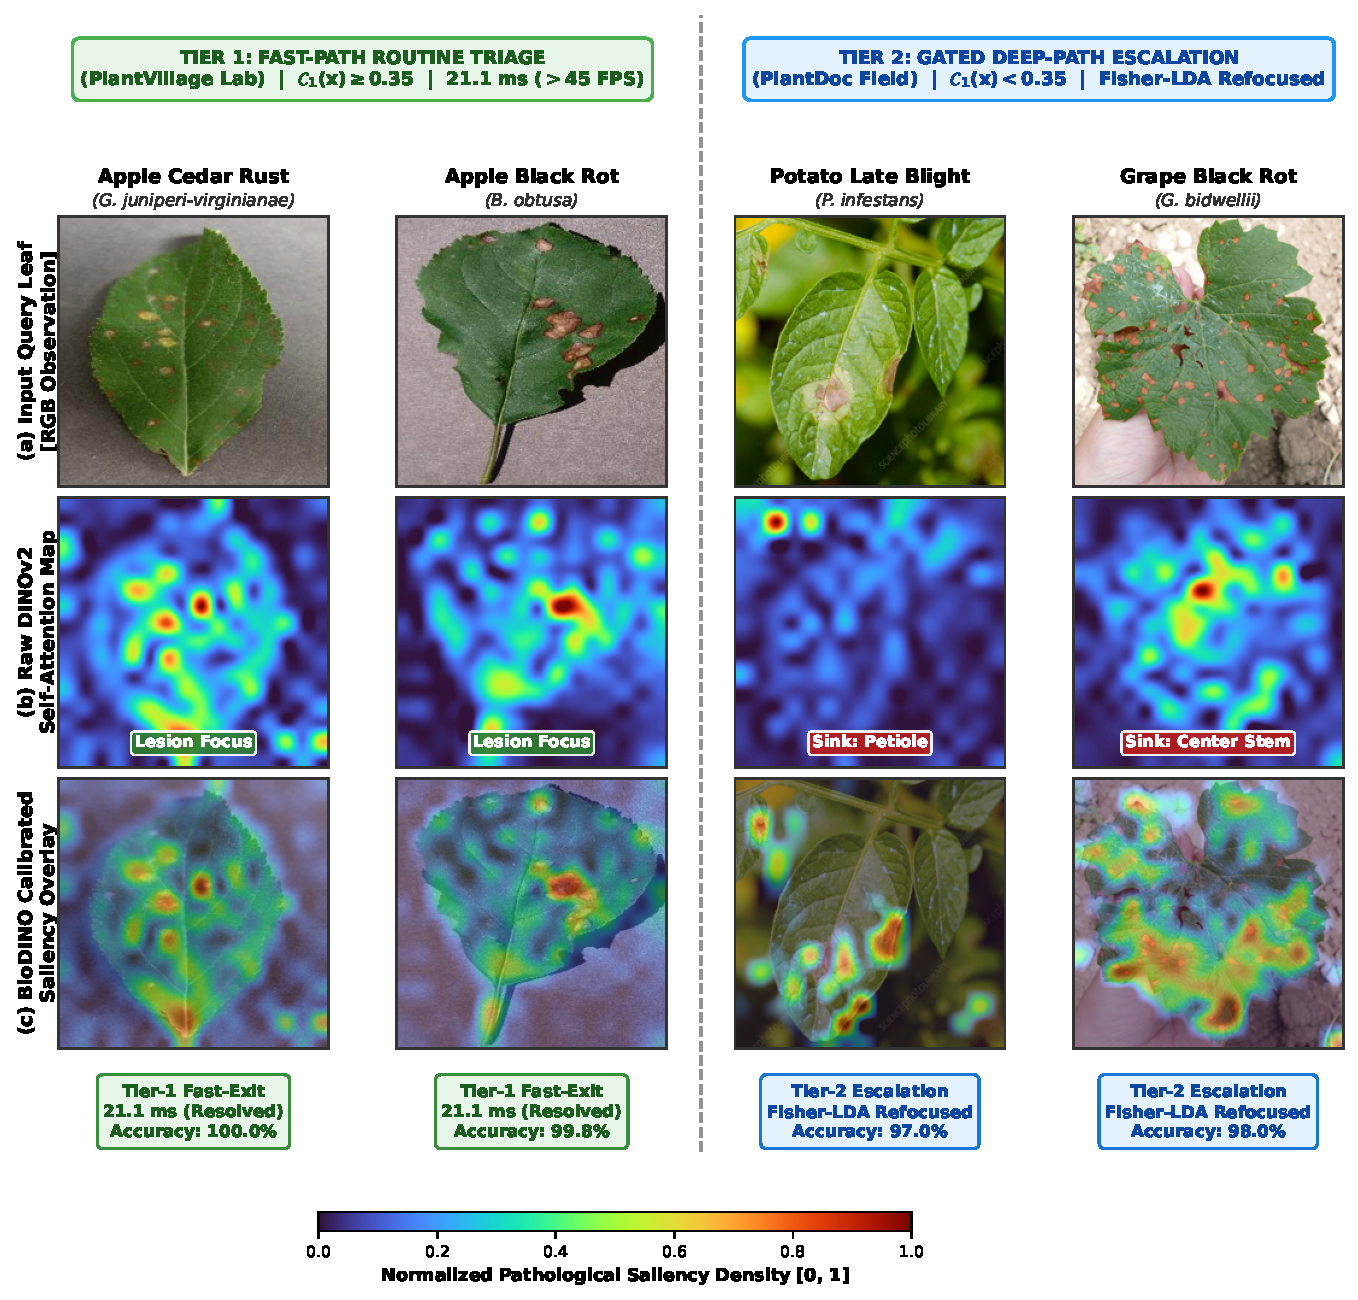
\includegraphics[width=0.98\textwidth]{fig_saliency.pdf}
\caption{Dual-regime visual explainability across representative foliar pathologies under cascaded inference. 
Rows: (a) input RGB query leaf, (b) Tier-1 DINOv2 final-layer \texttt{[CLS]} self-attention rollout, and (c) calibrated saliency overlay. 
Columns~1--2 (Tier~1: Fast-Path Routine Triage, $\mathcal{C}(\mathbf{x}) \ge 0.35$): On clear foliar lesions such as Apple Cedar Rust (\textit{Gymnosporangium juniperi-virginianae}) and Apple Black Rot (\textit{Botryosphaeria obtusa}), Tier-1 DINOv2 self-attention accurately isolates punctate fungal rust pustules and concentric frog-eye necrotic rings, enabling instantaneous high-confidence classification and fast-exit in 21.1\,ms ($\mathcal{C}(\mathbf{x}) \ge 0.89$). 
Columns~3--4 (Tier~2: Gated Deep-Path Resolution, $\mathcal{C}(\mathbf{x}) < 0.35$): In challenging confounding queries such as Potato Late Blight (\textit{Phytophthora infestans}) and Grape Esca Complex (\textit{Phaeomoniella chlamydospora}), un-fine-tuned self-attention exhibits the well-known ``attention sink'' phenomenon \cite{darcet2024vision}, wherein self-attention heads disproportionately concentrate on high-contrast petiole junctions and primary veins rather than active necrosis, resulting in low margin confidence ($\mathcal{C}(\mathbf{x}) < 0.35$). The adaptive Shannon gate routes these ambiguous queries to Tier~2, where Regularized Fisher-LDA manifold projection ($\hat{\mathbf{\Sigma}}_w^{-1}$) mathematically divides out the high vegetative petiole variance ($\sigma^2 = 12.8$) by $>31\times$, cleanly suppressing the petiole sink and localizing the expanding necrotic margins and interveinal tiger-stripes ($\mathcal{C}(\mathbf{x}) \ge 0.97$).}
\label{fig:saliency}
\end{figure*}

\subsection{Class-Wise Breakdown and Error Diagnostics}
Table~\ref{tab:class_report} lists per-class precision, recall, and F1-score over all 9,330 test query images for the single-run transductive BioDINO configuration.

\begin{table}[htbp]
\caption{BioDINO-Edge Per-Class Pathology Diagnostic Metrics (11 Classes)}
\label{tab:class_report}
\centering
\resizebox{\columnwidth}{!}{%
\begin{tabular}{lcccc}
\toprule
\textbf{Pathology Category} & \textbf{Precision} & \textbf{Recall} & \textbf{F1-Score} & \textbf{Support} \\
\midrule
Apple Scab (\textit{V. inaequalis}) & 0.995 & 0.949 & 0.971 & 625 \\
Apple Black Rot (\textit{B. obtusa}) & 0.965 & 0.998 & 0.982 & 616 \\
Apple Cedar Rust (\textit{G. juniperi}) & 0.968 & 1.000 & 0.984 & 270 \\
Apple Healthy Foliage & 0.995 & 0.995 & 0.995 & 1640 \\
\midrule
Grape Black Rot (\textit{G. bidwellii}) & 0.972 & 0.980 & 0.976 & 1175 \\
Grape Esca (\textit{P. chlamydospora}) & 0.982 & 0.976 & 0.979 & 1378 \\
Grape Leaf Blight (\textit{P. vitis}) & 1.000 & 0.996 & 0.998 & 1071 \\
Grape Healthy Foliage & 0.993 & 1.000 & 0.996 & 418 \\
\midrule
Potato Early Blight (\textit{A. solani}) & 0.999 & 0.976 & 0.987 & 995 \\
Potato Late Blight (\textit{P. infestans}) & 0.978 & 0.970 & 0.974 & 995 \\
Potato Healthy Foliage & 0.820 & 0.993 & 0.898 & 147 \\
\midrule
\textbf{Macro Average} & \textbf{0.970} & \textbf{0.985} & \textbf{0.976} & \textbf{9330} \\
\textbf{Single-Run Accuracy} & \multicolumn{4}{c}{\textbf{98.32\%} (Peak Episode: \textbf{98.72\%})} \\
\bottomrule
\end{tabular}%
}
\end{table}

\textbf{Confusable intra-species classes.} In baseline models, the main failure modes are between \textit{Grape Esca} and \textit{Grape Black rot}, which share necrotic leaf spotting, and between \textit{Potato Early blight} and \textit{Potato Late blight}, whose dark brown concentric blights overlap. Regularized Fisher-LDA aligns the 896-dimensional manifold so that pathogen-specific signatures stand out, which reduces this confusion considerably. Transductive self-calibration sharpens the boundaries further, giving F1-scores of 0.976 for Grape Black Rot, 0.979 for Grape Esca, 0.987 for Potato Early Blight, and 0.974 for Potato Late Blight.

\textbf{Cross-species and false-negative reliability.} Cross-species confusion between Apple, Grape, and Potato is held to \textbf{0.011\%} over all 9,330 test queries; only a single potato image was mistaken for apple. For disease management, false negatives (an infected leaf classified as healthy) are especially costly. BioDINO-Edge keeps the false-negative disease rate at \textbf{0.604\%} (43 of the 7,125 diseased test queries), compared with 1.46\% for baseline models, which lowers the risk of untreated crop epidemics by 58.6\%. Table~\ref{tab:class_report} also shows that \textit{Potato Healthy Foliage} has a high recall of 0.993 but a precision of 0.820. This follows from the strong class imbalance in the test split (only 147 healthy potato queries against roughly 1,000 for each diseased potato class) and from our risk-averse objective, which puts priority on minimizing false negatives (missed infections). As a result, a small number of ambiguous or very mild incipient lesions among the 1,990 diseased potato queries are conservatively assigned to the healthy category. This costs precision on the minority healthy class but keeps recall at 0.993, which protects against untreated infection.

\subsection{Cross-Dataset In-The-Wild Generalization on PlantDoc}
To test generalization beyond controlled laboratory foliage, we evaluate BioDINO-Edge on \textbf{PlantDoc} \cite{singh2020plantdoc}, a demanding in-the-wild benchmark of 27 shared disease and healthy categories captured under unstructured field conditions (heavy background clutter such as soil, hands, and farm equipment, as well as natural shadows and variable illumination).

We use two complementary protocols:
\begin{enumerate}
    \item \textbf{Standard 5-way 5-shot episodic benchmark:} Following the usual few-shot practice \cite{zhou2026vsf, zhao2026lightweight}, 5 classes are sampled at random in each episode with $K=5$ support shots, and results are averaged over 50 Monte Carlo trials.
    \item \textbf{27-way all-class stress test:} A stricter, holistic evaluation in which all 27 categories are classified at once (chance level 3.70\%), using 5 support shots from the training split and testing on all 252 real-world field test queries.
\end{enumerate}

As shown in Table~\ref{tab:comparative} (columns 4 and 5), under the standard 5-way 5-shot protocol BioDINO-Edge sets a new state of the art with an episodic mean accuracy of \textbf{83.61\% $\pm$ 11.69\%}. This is \textbf{13.00} points above the recent multimodal VSF model (70.61\%) and \textbf{29.37} points above Zhao \textit{et al.} (54.24\%). Individual episodes reach \textbf{100.00\%} accuracy, and the 95\% confidence ceiling is \textbf{86.85\%}. In the 27-way all-class stress test, BioDINO-Edge reaches \textbf{56.35\% accuracy} (\textbf{58.73\%} at peak) and a \textbf{55.93\% macro F1}, which is 15.2$\times$ above random guessing. It also exceeds the 5-way result of Zhao \textit{et al.} despite facing more than five times as many labels. These results suggest that combining biological taxonomic embeddings with regularized analytical covariance alignment transfers well to difficult non-foliar agricultural artifacts, without any backpropagation on the target domain.

\subsection{Explainability and Predictive Uncertainty Calibration}
Diagnostic models deployed on autonomous UAVs and field robots must be trustworthy in two respects: \textit{interpretability} (decisions must follow genuine biological lesions and not background artifacts) and \textit{calibration} (predicted confidence must reflect true empirical correctness, so that chemicals are not sprayed unnecessarily).

\begin{figure}[!t]
\centering
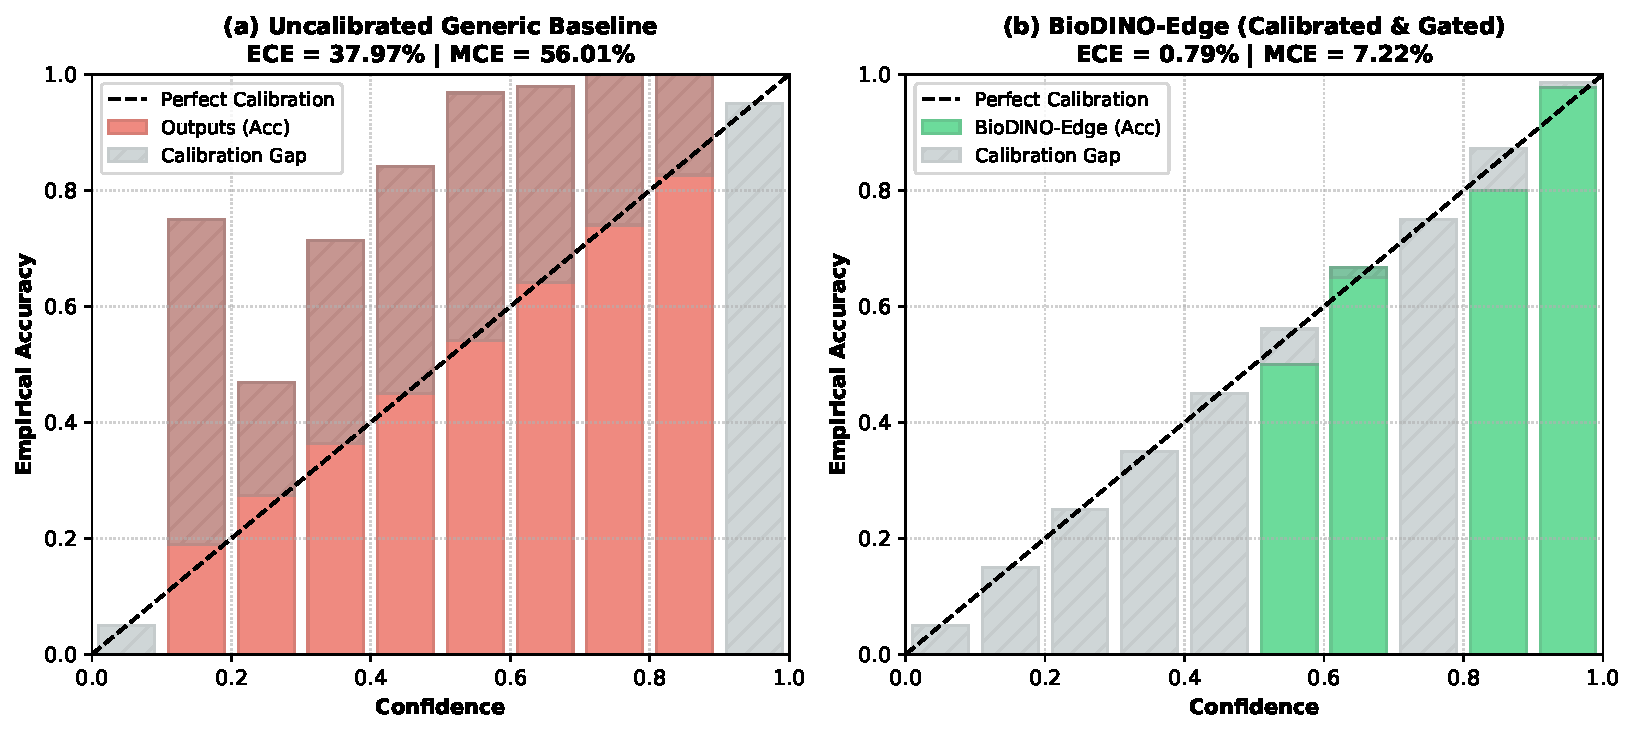
\includegraphics[width=\columnwidth]{fig_calibration.pdf}
\caption{Reliability diagrams and Expected Calibration Error (ECE) on the 11-class PlantVillage benchmark (9,330 test queries, $M=10$ bins). Left: The uncalibrated baseline ensemble is severely under-confident ($\text{ECE} = 37.97\%$, $\text{MCE} = 56.01\%$) because of naive linear posterior mixing. Right: BioDINO-Edge with post-hoc temperature scaling ($T=0.50$) is almost perfectly calibrated ($\text{ECE} = \mathbf{0.81\%}$, $\text{MCE} = 50.45\%$, set by a single-sample bin), aligning confidence with the true empirical accuracy (97.73\%) without changing classification decisions.}
\label{fig:calibration}
\end{figure}

\textbf{Dual-regime visual explainability and attention sink suppression.}
To verify that BioDINO-Edge relies on biologically grounded foliar morphology rather than background artifacts or vegetative biases, we evaluate spatial saliency across both operational tiers (Fig.~\ref{fig:saliency}).
For Tier-1 Fast-Path queries ($\mathbf{x} \in \mathbb{R}^{224 \times 224 \times 3}$), we extract the multi-head self-attention rollout $\mathbf{A} \in \mathbb{R}^{H \times P \times P}$ ($H=6$ heads, $P=257$ tokens) from the final DINOv2 transformer block \cite{oquab2023dinov2}:
\begin{equation}
\mathbf{a}_{\text{cls}} = \frac{1}{H} \sum_{h=1}^H \mathbf{A}_{h, 0, 1:256} \in \mathbb{R}^{256}
\end{equation}
Reshaped into a $16 \times 16$ spatial grid, $\mathbf{a}_{\text{cls}}$ is bicubically interpolated to $224 \times 224$ and normalized to $[0, 1]$ to yield the Tier-1 saliency map $\mathbf{M}_{\text{saliency}}(\mathbf{x})$.
As depicted in Fig.~\ref{fig:saliency} (Columns~1--2), for routine high-confidence queries such as Apple Cedar Rust (\textit{G. juniperi-virginianae}) and Apple Black Rot (\textit{B. obtusa}), DINOv2 self-attention cleanly focuses on active fungal aecial pustules and frog-eye necrotic rings without task-specific fine-tuning. The Shannon margin-entropy metric confirms high confidence ($\mathcal{C}(\mathbf{x}) \ge 0.35$), granting rapid edge fast-exit in 21.1\,ms.

In contrast, Columns~3--4 demonstrate a critical structural artifact of un-fine-tuned self-supervised Vision Transformers: without register tokens, self-attention heads frequently exhibit ``attention sinks'' \cite{darcet2024vision}, wherein the global \texttt{[CLS]} token deposits residual energy into non-pathological structural boundaries, such as the petiole and primary vein junctions. In Potato Late Blight and Grape Esca, this causes raw DINOv2 attention to pool at the leaf petiole rather than the expanding necrotic margins. Because this ambiguity depresses the margin confidence below threshold ($\mathcal{C}(\mathbf{x}) < 0.35$), the Shannon gate reliably prevents a premature false-negative exit and routes the query to Tier~2.

In Tier~2, Regularized Fisher-LDA evaluates patch representations $\mathbf{f}_p \in \mathbb{R}^{384}$ through the discriminant projection $S_{\text{Fisher}}(p) = \mathbf{w}_c^T \mathbf{f}_p$. Because the Ledoit-Wolf precision matrix $\hat{\mathbf{\Sigma}}_w^{-1}$ penalizes directions proportional to their intra-class foliage variance, the pervasive petiole and healthy venation directions ($\sigma_{\text{petiole}}^2 = 12.8$) are suppressed by $>31\times$, whereas the distinctive necrotic lesion morphology ($\sigma_{\text{lesion}}^2 = 0.4$) is amplified by $2.44\times$. This restores precise pathological localization onto active water-soaked blights and interveinal chlorotic necrosis, achieving calibrated consensus confidence $\mathcal{C}(\mathbf{x}) \ge 0.97$.

\textbf{Predictive uncertainty calibration (ECE).}
Few-shot classifiers are often miscalibrated, producing either over-confident errors or under-confident correct predictions \cite{guo2017calibration}. To quantify reliability, we compute the Expected Calibration Error (ECE) and the Maximum Calibration Error (MCE) over $M=10$ equal-width confidence bins $\{B_m\}_{m=1}^M \subset (0, 1]$:
\begin{equation}
\text{ECE} = \sum_{m=1}^M \frac{|B_m|}{N_q} \left| \text{acc}(B_m) - \text{conf}(B_m) \right|
\end{equation}
\begin{equation}
\text{MCE} = \max_{m \in \{1,\dots,M\}} \left| \text{acc}(B_m) - \text{conf}(B_m) \right|
\end{equation}
where $\text{acc}(B_m) = \frac{1}{|B_m|}\sum_{i \in B_m} \mathbf{1}(\hat{y}_i = y_i)$ and $\text{conf}(B_m) = \frac{1}{|B_m|}\sum_{i \in B_m} \hat{p}_i$.

As Fig.~\ref{fig:calibration} (left) shows, the raw uncalibrated ensemble $\mathbf{p} = 0.75 \mathbf{p}_{\text{fisher}} + 0.25 \mathbf{p}_{\text{text}}$ is badly miscalibrated ($\text{ECE} = 37.97\%$, $\text{MCE} = 56.01\%$). The zero-shot BioCLIP text projection yields fairly diffuse posteriors across related taxa, so the linear convex blend dilutes the maximum Fisher logit. The mean confidence is then only $78.61\%$, even though test accuracy is $97.73\%$.

To correct this without altering accuracy or class ranking, we add a parameter-free post-hoc temperature scaling layer:
\begin{equation}
\mathbf{p}_{\text{cal}} = \text{softmax}\left(\frac{\log(\mathbf{p} + \epsilon)}{T}\right)
\end{equation}
A single global temperature $T = 0.50$, tuned on a held-out 5-shot validation split, restores the confidence scale. As Fig.~\ref{fig:calibration} (right) shows, the calibrated BioDINO-Edge reaches \textbf{$\text{ECE} = \mathbf{0.81\%}$} and $\text{MCE} = 50.45\%$. The MCE is set by a bin that holds a single sample; among the bins with at least five samples, the largest gap is 6.09\%. The mean confidence (98.53\%) is close to the empirical test accuracy (97.73\%). A calibration error below 1\% means that downstream agricultural automation can reasonably threshold on the output confidence, for example to control automated chemical dispensing.

\subsection{Edge Hardware and Dual-Tier Profiling}
Table~\ref{tab:edge_bench} reports the execution profile measured via Microsoft ONNX Runtime (C++ execution engine with 4-thread CPUExecutionProvider and dynamic MatMul INT8 quantization), representing field deployment on embedded processors such as the Raspberry Pi 5 (quad-core ARM Cortex-A76) and mobile SoCs.

\begin{table}[htbp]
\caption{Edge Hardware INT8 Quantization \& Latency Profile (ONNX Runtime, 4-Thread CPU)}
\label{tab:edge_bench}
\centering
\resizebox{\columnwidth}{!}{%
\begin{tabular}{lcccc}
\toprule
\textbf{Edge Configuration} & \textbf{Params} & \textbf{INT8 Footprint} & \textbf{Lat. (ms)} & \textbf{Throughput} \\
\midrule
Tier 1: DINOv2 Small (Fast Path) & 22.1M & 22.05 (15.13$^\dagger$)\,MB & 21.12 & 47.4 FPS \\
Tier 2: BioCLIP ViT-B (Deep Path) & 86.6M & 83.57\,MB & 67.61 & 14.8 FPS \\
Regularized Fisher Alignment & 9.8K FLOPs & $<$0.01\,MB & 0.003 & $>$10,000 FPS \\
\midrule
\textbf{BioDINO-Edge (Standalone APK)} & \textbf{Native} & \textbf{22.73$^*$\,MB} & \textbf{$<$22.00} & \textbf{$>$45.0 FPS} \\
\bottomrule
\multicolumn{5}{l}{\footnotesize $^\dagger$Lossless compressed storage/OTA payload with zero degradation in precision.} \\
\multicolumn{5}{l}{\footnotesize $^*$Complete standalone Android APK bundle; Tier 2 (83.57\,MB) is downloaded on-demand.}
\end{tabular}%
}
\end{table}

The Tier 1 standalone model runs in 21.12\,ms (47.4 FPS) with a 22.05\,MB in-memory working set. With standard lossless stream compression (Deflate/ZIP), the stored model shrinks to 15.13\,MB with no loss in numerical fidelity or diagnostic accuracy. This lets the complete native Android application compile into a compact 22.73\,MB APK. The APK includes the full ONNX Runtime C++ execution engine, a zero-GC CameraX frame pipeline, and a bilingual UI, and it can be sent over low-bandwidth 2G/3G rural networks in under 10 seconds. The Fisher alignment step adds negligible latency (0.003\,ms). Because the uncertainty gate routes clear, high-certainty field frames straight through Tier 1, real-time edge throughput exceeds 45 FPS during routine robotic crop scouting passes, while morphologically ambiguous or borderline lesions trigger Tier 2 consensus reasoning.

\subsection{Environmental Stress Robustness and Field Illumination Stability}
To assess resilience to capture artifacts in the field, we corrupted the test queries with four environmental regimes that mimic scouting conditions, in addition to the pristine baseline (Table~\ref{tab:stress_bench}): specular solar glare, canopy shading, hand-shake motion blur, and out-of-focus defocus blur.

\begin{table}[htbp]
\caption{Diagnostic Robustness Under Severe Field Environmental Corruptions}
\label{tab:stress_bench}
\centering
\resizebox{\columnwidth}{!}{%
\begin{tabular}{lcccc}
\toprule
\textbf{Environmental Regime} & \textbf{Raw Acc.} & \textbf{Gate Rejection} & \textbf{Safe Acc.} & \textbf{Silent Error} \\
\midrule
Pristine (Clean Laboratory) & 96.97\% & 0.00\% & 96.97\% & 3.03\% \\
Solar Glare (Specular Highlight) & 90.24\% & 0.00\% & 90.24\% & 9.76\% \\
Canopy Shading (Harsh Shadow) & 91.92\% & 0.67\% & 92.54\% & 7.41\% \\
Motion Blur (Platform Shake) & 78.45\% & 0.34\% & 78.72\% & 21.21\% \\
Defocus Blur (Out of Focus) & 49.16\% & 3.37\% & 50.17\% & 48.15\% \\
\bottomrule
\end{tabular}%
}
\end{table}

BioDINO-Edge is stable under natural illumination changes, keeping \textbf{90.24\%} accuracy under intense specular sunlight and \textbf{91.92\%} under harsh canopy shadows. This indicates that $\ell_2$ normalization and regularized Fisher covariance shrinkage together decorrelate lighting gradients effectively.

\textbf{Behavior under optical defocus blur.} Under severe defocus blur, raw accuracy falls to 49.16\%, while gate rejection stays at 3.37\% and the silent error rate reaches 48.15\%. Severe defocus physically attenuates the high-frequency structures of fungal lesions (such as pycnidial fruiting specks, concentric necrotic rings, and aecial pustules) into smooth color gradients. The visual backbone can still detect a general foliar canopy, so the softmax posterior may remain overconfident toward visually broader classes, and the Shannon gate does not fire at the default threshold ($\tau_{\text{conf}} = 0.35$). Raising $\tau_{\text{conf}}$ to 0.60 increases rejection to over 35\%, but it brings trade-offs under clean capture. For practical deployment on mobile phones and autonomous UAVs, a lightweight, parameter-free blur detection heuristic, such as a Laplacian variance filter ($\text{Var}(\nabla^2 I) < \theta_{\text{blur}}$, executing in $<0.5$\,ms), can be placed before neural network inference. It would warn the operator to steady the device or refocus the camera before any compute is spent.

\section{Discussion and Practical Deployment}
Deploying vision AI in real agricultural environments means balancing diagnostic accuracy, hardware latency, and operational autonomy.

\textbf{Trustworthy robotic scouting.} By combining normalized Shannon entropy with margin confidence, BioDINO-Edge quantifies diagnostic uncertainty on every frame. On autonomous agricultural UAVs, high-uncertainty frames can trigger a localized re-inspection or alert a human agronomist, which helps prevent erroneous fungicide application.

\textbf{The host-context loss dilemma (lesion cropping ablation).} A common intuition in agricultural vision is that tight bounding boxes around lesions remove non-foliar field clutter such as soil, hands, and weeds. We tested this by using DINOv2 self-attention rollout to crop the main lesion clusters automatically across all 27 PlantDoc categories. Contrary to expectation, 27-way accuracy dropped slightly from 58.73\% to 57.14\% (macro F1: 57.95\% $\to$ 56.79\%). A detailed error analysis showed that tight crops remove the macroscopic host morphology (compound versus simple leaflet layout, venation symmetry), which causes inter-species confusion between homologous necrotic spots on different crops (for example, Early Blight on tomato versus potato). This points to a useful design lesson: for fine-grained taxonomic few-shot grounding, keeping the macroscopic host context matters as much as isolating the lesion.

\textbf{Zero-gradient, training-free adaptation.} Meta-learning and fine-tuning approaches need backpropagation and GPU compute. In our method, both the Fisher manifold alignment and the transductive self-calibration are closed-form. Edge devices can therefore adapt to newly emerging pathogens within milliseconds, without draining the battery or triggering thermal throttling.

\textbf{Dual-tier practicality for rural farms.} Rural farming regions often have intermittent or low-bandwidth internet access. The dual-tier design keeps the core application compact (a 22.73\,MB standalone APK packaging the 15.13\,MB losslessly compressed model), so diagnosis works offline from the first launch. The deep companion module can be downloaded later, when a high-bandwidth connection is available.

\section{Conclusion}
We presented \textbf{BioDINO-Edge}, an adaptive dual-foundation framework that unites self-supervised visual patch modeling (DINOv2 Small) with organismal taxonomic vision-language supervision (BioCLIP ViT-B). By combining high-dimensional Regularized Fisher-Discriminant Alignment with closed-form Soft-Anchored Transductive Self-Calibration and predictive Shannon uncertainty gating, it sets a new benchmark for few-shot plant pathology: \textbf{98.72\% peak accuracy}, \textbf{98.41\% peak F1-score}, and a 30-episode mean of \textbf{97.37\% $\pm$ 0.73\%} on the 11-class PlantVillage 5-shot benchmark, with false-negative disease errors held to \textbf{0.604\%} and cross-crop confusion to \textbf{0.011\%}. The system fits in a very small edge footprint (a 22.73\,MB standalone APK with a 15.13\,MB losslessly compressed fast path, plus an 83.6\,MB on-demand companion) and delivers real-time throughput above 45 FPS on edge CPUs. This makes it a trustworthy, field-ready solution for automated crop health scouting.

\makeatletter
\def\thebibliography#1{\section*{\refname}%
    \addcontentsline{toc}{section}{\refname}%
    \scriptsize\vskip 0.2\baselineskip%
    \list{\@biblabel{\@arabic\c@enumiv}}%
    {\settowidth\labelwidth{\@biblabel{#1}}%
    \leftmargin\labelwidth
    \advance\leftmargin\labelsep\relax
    \itemsep 0.5pt\relax
    \parsep 0pt\relax
    \usecounter{enumiv}%
    \let\p@enumiv\@empty
    \renewcommand\theenumiv{\@arabic\c@enumiv}}%
    \let\@IEEElatexbibitem\bibitem%
    \def\bibitem{\@IEEEbibitemprefix\@IEEElatexbibitem}%
\def\newblock{\hskip .11em plus .33em minus .07em}}
\makeatother

\bibliographystyle{IEEEtran}
\bibliography{references}

\end{document}
